\chapter{Harmonic Excitation}
\label{chap:Excitation}

\section{Introduction}
\label{sec:Excitation-Introduction}
	Nonlinear distortion is an inherent part of an analogue signal path. It alters the dynamic variation of signals and
	introduces new spectral components. Its use as a creative effect is best known by guitar players due to the use of
	values in early guitar amplifiers imparting nonlinear transforms onto the audio signal
	\citep{dutilleux2011nonlinear}. This distorted sound became desirable and several electronic circuits were developed
	with the purpose of inducing nonlinear distortion. More recently, research into modelling these distortion circuits
	in the digital domain has been carried out, such as that done by \citet{pakarinen2009a}. Several researchers have
	also worked on creating novel digital distortion techniques \citep{fernandez-cid2001distortion, puckette2007patch,
	pekonen2008coefficient}.

	Distortion is a very broad term which is often used to describe unwanted effects. For this work a better defined
	term, harmonic excitation, will be used to refer to the deliberate and controlled application of nonlinear systems
	in order to introduce new frequency components to a signal. \citet{dutilleux2011nonlinear} defines excitation as the
	process of controlling timbre through the emphasis of certain frequencies. While this is possible with linear
	systems such as equalisers, nonlinear systems provide more flexibility as they can add energy in areas of the
	spectrum where the original signal had none.

	This chapter will review how nonlinear systems have been analysed in previous audio research, how their effects are
	quantified and the timbral transforms they impart. Firstly the analysis of nonlinear systems is discussed in Section
	\ref{sec:Excitation-AnalysisOfNonlinearSystems}. Existing research into the perceived timbral effects of these
	systems is then discussed in Section \ref{sec:Excitation-Timbre}. Section \ref{sec:Excitation-Uses} describes the
	common uses for nonlinear distortion by audio engineers. Section \ref{sec:Excitation-Methods} then explains the
	operation of various nonlinear systems used, or proposed for use, in audio processing.

\section{Analysis of Nonlinear Systems}
\label{sec:Excitation-AnalysisOfNonlinearSystems}
	The behaviour of an LTI system can be entirely summarised by its response to an impulse signal
	\citep{phillips2007signals}. Once the impulse response of the system has been measured, the system's response to any
	arbitrary input is known. Analysis of nonlinear systems is more complicated, unlike LTI systems the properties of
	the system cannot be summarised by the system's response to a single input signal. Depending on the field in which a
	nonlinear system is being studied, different approaches are taken in an attempt to summarise the behaviour of
	nonlinear systems. In the field of audio engineering much of the literature concerning nonlinearities has to do with
	minimising distortion or measuring the maximum allowable levels of distortion. Several distortion metrics have been
	developed each with their own uses. A review of many of these metrics is given by \cite{voishvillo2006assessment},
	some of which will be discussed in Section \ref{sec:Excitation-Analysis-Metrics}. Where more information is needed,
	nonlinear modelling techniques are used. These typically involve setting the parameters of a generalised nonlinear
	system such that its behaviour matches that of the system being analysed. The nonlinear modelling techniques
	utilised in the audio processing literature are discussed in Section \ref{sec:Excitation-Analysis-Modelling}. Prior
	to discussing how the effects of nonlinear systems are measures / modelled the concept of distortion components (the
	artefacts introduced by nonlinear systems) is introduced in Section \ref{sec:Excitation-Analysis-Components}.

	\subsection{Distortion Components}
	\label{sec:Excitation-Analysis-Components}
		Nonlinear systems introduce new spectral components to a signal. These distortion components are produced
		via intermodulation of the existing components in the signal. The frequencies of these distortion components
		are linear combinations of the frequency components in the input signal. For a signal with $N$ frequency
		components each possible distortion component takes the form of Equation \ref{eq:IntermodulationComponents}.

		\begin{equation}
			f = \sum_{n = 1}^{N} k_{n}f_{n}, \quad k_{n} \in \textbf{Z}
			\label{eq:IntermodulationComponents}
		\end{equation}

		Where $f_{n}$ is the frequency of the $n$\super{th} frequency component of the input signal and each $k_{n}$
		an arbitrary integer scaling factor.

		The order of the distortion component, $O$, is calculated as the sum of the absolute values of these scaling
		factors (Equation \ref{eq:IntermodulationOrder}).

		\begin{equation}
			O = \sum_{n = 1}^{N} \abs{k_{n}}
			\label{eq:IntermodulationOrder}
		\end{equation}

		The exact distortion components introduced are determined by the input signal and the system used to process
		it. The components introduced can be ascribed to two different groups:

		\subsubsection*{Harmonic Distortion}
			Harmonic distortion refers to the distortion components generated by a signal's frequency components
			modulating themselves. This refers to the situation where all but one of the scaling factors in
			Equation \ref{eq:IntermodulationComponents} are zero. The frequencies of every harmonic distortion
			component are integer multiples of a frequency component in the original signal. 
			
			For a sinusoidal input only harmonic distortion components are generated. The number of harmonic
			distortion components introduced grows linearly with the number of frequency components in the input
			signal.

		\subsubsection*{Intermodulation Distortion}
			Intermodulation distortion refers to distortion components introduces when two or more of the
			spectral components in a signal modulate each other. If all the components in the input are
			harmonically related the intermodulation components will also lie at harmonic frequencies. A signal
			with slight inharmonicities in it will produce intermodulation components which amplify these
			inharmonicities.

			The number of intermodulation components grows exponentially as the number of frequency components
			in the input increases. This makes it more difficult to predict the intermodulation characteristics
			of a system.

		\subsubsection*{Aliasing}
			In a digital system frequency components of a signal are subject to aliasing. Aliasing arises due
			to the discrete nature of digital audio signals. The sampling frequency of a discrete signal imposes
			a restriction on the highest frequency which can be represented. This frequency is known as the
			Nyquist frequency ($f_{N}$) and can be calculated using Equation \ref{eq:nyquist}.

			\begin{equation}
				f_{N} = \frac{f_{s}}{2}
				\label{eq:nyquist}
			\end{equation}

			Where $f_{s}$ is the sampling rate of the signal.

			When sampling a signal, frequency content above the Nyquist is represented as alias frequencies
			within the bandwidth allowed by the sampling frequency. The alias frequency can be calculated using
			Equation \ref{eq:aliasing}.

			\begin{equation}
				f_{alias} = \abs{f - f_{s}\floor{\frac{f}{f_{s}} + \frac{1}{2}}}
				\label{eq:aliasing}
			\end{equation}

			Where $f$ is the original frequency.

			The new frequency content introduced to a discrete signal via nonlinear processing is also subject
			to aliasing. This can cause problems in the uniformity of behaviour of a system in different
			scenarios as the spectral content introduced will depend on the sampling frequency of the signal
			being processed. Thus, the perceived timbral transform may also depend on the sampling frequency.

			There are two various methods for avoiding unwanted aliasing distortion in nonlinear effects.

			\citep{vetter2013estimation} upsample signals by a factor of 32 prior to applying the nonlinearity.
			Afterwards the signal is downsampled to the original sampling frequency. This method relies on the
			use of a nonlinearity which produces harmonics whose amplitudes decrease as their frequencies
			increase. This way upsampling can be applied such that only the low amplitude, high frequency,
			partials are aliased. The upsampling factor can be chosen such that these aliased partials are
			rendered inaudible.

			Upsampling does however increase the computational complexity of the system. Along with the extra
			overhead of upsampling and downsampling the signal, there is also a larger number of samples to
			process.

			For certain excitation methods it may be possible to reduce aliasing by changing properties of the
			processing algorithm. Details of these techniques will be discussed where appropriate in Section
			\ref{sec:ExcitationEvaluation-Comparison}.

	\subsection{Objective Distortion Metrics}
	\label{sec:Excitation-Analysis-Metrics}
		Total Harmonic Distortion (THD) and Intermodulation Distortion (IMD) are the traditional objective measures
		of distortion \citep{czerwinski2001multitone1}. 
		
		THD measures the level of new harmonic components introduced to a sinusoidal signal. There are two different
		ways in which THD is calculated. These have been denoted THD\sub{F} and THD\sub{R} by
		\citet{shmilovitz2005on} and are calculated using Equations \ref{eq:thdf} and \ref{eq:thdr} respectively.

		\begin{equation}
			\textrm{THD}_{\textrm{F}} = \frac{\sqrt{\sum_{n = 2}^{\infty} a_{n}^{2}}}{a_{1}}
			\label{eq:thdf}
		\end{equation}

		\begin{equation}
			\textrm{THD}_{\textrm{R}} = \sqrt{\frac{\sum_{n = 2}^{\infty} a_{n}^{2}}
			                                       {\sum_{n = 1}^{\infty} a_{n}^{2}}}
			\label{eq:thdr}
		\end{equation}

		Where $a_n$ is the amplitude of the $n$\super{th} harmonic. 

		Each of these measures has slightly different properties. THD\sub{R} measure the proportion of the output
		signal which consists of new harmonic components, producing a value between zero and one. THD\sub{F}
		measures the relative levels of new harmonic content and the energy at the frequency of the original
		sinusoid producing a positive value. \citet{shmilovitz2005on} suggests that THD\sub{F} provides a better
		measure for signals with high distortion as there is no upper bound on the value which is produced.

		Both these methods been used in recent work published in the audio field (THD\sub{F} by
		\citet{fleischmann2014a} and THD\sub{R} by \citet{dutilleux2011nonlinear}). The lack of standardisation for
		this metric makes it difficult to compare experimental results reported by different sources.

		Various standards exists for the measurement of IMD. Typically the systems response to a signal consisting
		of two sinusoids is measured. According to the \citet{IEC2001amplifiers} standard, a signal comprising two
		frequency components, $f_{1}$ and $f_{2}$ (where $f_{2} > f_{1}$), with an amplitude ratio of 4:1 is used.
		The only the levels of the second and third order intermodulation components are then measured separately
		according to Equations \ref{eq:imd2} and \ref{eq:imd3}.

		\begin{equation}
			\textrm{IMD}_{2} = 100\frac{a_{f_{2} + f_{1}} + a_{f_{2} - f_{1}}}{a_{f_{2}}}
			\label{eq:imd2}
		\end{equation}

		\begin{equation}
			\textrm{IMD}_{3} = 100\frac{a_{f_{2} + 2f_{1}} + a_{f_{2} - 2f_{1}}}{a_{f_{2}}}
			\label{eq:imd3}
		\end{equation}

		Where $a_{f}$ is the amplitude of frequency $f$ in the output signal.

		THD and IMD give very limited information about the response of nonlinear systems. They are typically
		measured using simple input signals which are not representative of the signals a system would process in
		actual use. Given that nonlinear systems may not satisfy the condition of superposition a system may
		process simple and complex signals in vastly differing manners. 

		These metrics also give no indication of the perceived degradation in audio quality a system introduces. A
		signal with a high THD values may potentially sound less distorted that one with a small THD. Several
		researchers have developed new distortion metrics which indicate the perceived amount of distortion.

		\citet{geddes2003auditory} suggest some psychoacoustic principles which may be applicable to the analysis
		of nonlinear distortion:

		\begin{itemize}
			\item New frequency components introduced, with lower frequencies than the original components,
				will be more perceptible.
			\item Higher order nonlinearity artefacts will be more perceptible.
			\item Nonlinearities which affect lower amplitude signals will be more perceptible.
		\end{itemize}

		\citet{voishvillo2006assessment} adds that the perception of distortion is decreased at the very high and
		low ends of the frequency spectrum.

		A subset of nonlinear systems can be described by a characteristic curve (a function mapping the
		instantaneous amplitude of the input signal to the input amplitude of the output signal). These systems are
		referred to as static nonlinearities and are memoryless systems (their behaviour is only governed by the
		instantaneous amplitude of the input, not any of its previous states).

		The GedLee metric, proposed by \citet{geddes2003auditory}, measures how much a static nonlinearity will be
		perceived through analysis of its characteristic curve. It is calculated using Equation \ref{eq:gedlee}.

		\begin{equation}
			G_{m} = \sqrt{\int_{-1}^{1} \left( \cos \left( \frac{x\pi}{2} \right) \right)^{2}
				      \left( \frac{d^{2}}{dx^{2}} T(x) \right)^{2} dx}
			\label{eq:gedlee}
		\end{equation}

		Where $T(x)$ is the characteristic curve of the static nonlinearity in question.

		A considerable advantage of the GedLee metric is that it directly measures the system in question rather
		than signals processed by it. This should allow measurements taken using the metric to describe the audible
		degradation of any signal processed by a system. \citet{lee2003auditory} provide results of an experiment
		in which their metric was tested against THD and IMD as a rating of audio quality. They show that for low
		levels of distortion the GedLee metric correlates with subjective audio quality ratings. THD and IMD are
		both found to not correlate well with perceived quality.

		The GedLee metric is only applicable to the analysis of static nonlinearities. Many nonlinear systems are
		more complex than this and may exhibit frequency dependant or time varying behaviour.  While the GedLee
		metric may provide a good, signal independent, measure of distortion, it is only applicable to a subset of
		nonlinear systems.

		\citet{tan2003the} also developed a perceptual metric for distortion, Distortion Score (DS), which they then
		improved upon to create the R\sub{nonlin} metric \citep{tan2004predicting}. Both these metrics rely on
		analysing signals which have been processed, so they may not give results which can be applied as generally
		as those using the GedLee metric. These metrics have an advantage in that they use models of the human
		hearing system to better approximate the perceived level of distortion.

		To calculate the DS the audio is split into frequency bands which model the auditory filters of the
		cochlear. These auditory filters represent bands within which two tones will interfere with the perception
		of each other \citep{fastl2007psychoacoustics}. Tones can be masked (made inaudible) by other tones within
		the same auditory filter band. By processing the audio in this manner the DS metric can take account of
		elements of the distortion which may not be perceptible because of masking.
		
		The R\sub{nonlin} metric improves on this model of the hearing system by including a filter with a
		frequency response similar to that of the outer and middle ear. The filter used is as described by
		\citet{glasberg2002a}, it attenuates frequencies at either end of the audible spectrum. This models the
		decreased perception of distortion at these frequencies as reported by \citet{voishvillo2006assessment}.

		\citet{tan2004predicting} report greater correlation between R\sub{nonlin} and perceived audio quality then
		\citet{lee2003auditory} do for the GedLee metric. They also demonstrate how accurate the R\sub{nonlin}
		metric is in predicting the perceived distortion level introduced to music and speech signals.

		The research discussed in this section has focused on measuring the extent to which unwanted distortion can
		be perceived. This does not provide enough information for the description of timbre. The listening tests
		performed to verify the developed metrics asked subjects to rate the quality of audio stimuli. It is
		possible that nonlinear distortion could alter the timbre of audio without deteriorating its perceived
		quality. Listeners could be asked to describe the timbre of different nonlinear distortions further rather
		than ranking them on the same distortion scale. Previous research has been carried out into the timbre of
		distortion as discussed in Section \ref{sec:Excitation-Timbre}.

	\subsection{Nonlinear Modelling}
	\label{sec:Excitation-Analysis-Modelling}
		Various techniques for modelling nonlinear systems have been developed in the mathematics and engineering
		literature. These models allow for more in depth analysis of a system as well as replicating its effects in
		the digital domain. Summaries of some of these modelling techniques can be found in the work by
		\citet{janczak2005identification} and \citet{ogunfunmi2007adaptive}.

		Two nonlinear modelling techniques have found use in audio processing:

		\begin{itemize}
			\item Wave Digital Filters as discussed by \citet{fettweis1986wave}.
			\item The Synchronised Swept Sine Method as described by \citet{novak2010nonlinear}.
		\end{itemize}

		These techniques are summarised here.

		\subsubsection{Wave Digital Filters}
			Wave digital filters are a class of filter which can be used to emulate analogue circuits. The
			process of creating a digital representation of a circuit involves constructing a `tree' of blocks.
			These blocks represent either electronic components, or connections between components in a
			circuit. Each block obeys a certain set of rules when presented with a signal. Blocks have been
			developed for modelling nonlinear circuit elements such as operational amplifiers and diodes
			\citep{paiva2012emulation}.

			While wave digital filters can accurately represent a nonlinear system, there are some
			disadvantages. As systems get more complex traversing the `tree' of blocks in order to calculate
			the output signal takes more computation. This presents problems when real time system response is
			needed. There are also certain circuit topologies which cannot be represented in the wave digital
			domain \citep{valimaki2011virtual}. Another consideration is that knowledge of the circuitry inside
			a system being modelled is needed. This might not always be available.

		\subsubsection{The Synchronised Swept Sine Method}
			The synchronised swept sine method is a technique for identifying nonlinear systems without prior
			knowledge of their operation. A nonlinear impulse response is generated by analysing the system's
			response to a signal with exponentially increasing frequency as described by
			\citet{novak2010nonlinear}. The result of the analysis is a series of filter kernels to be used in
			the model shown in Figure \ref{fig:hammerstein}.

			\begin{figure}[h!]
				\centering
				\begin{tikzpicture}
					\node (Sig2) [draw] at (1, 3) {$x[n]^{2}$};
					\node (Sig3) [draw] at (1, 2) {$x[n]^{3}$};
					\node (SigN) [draw] at (1, 0.5) {$x[n]^{N}$};

					\node (Filter1) [draw] at (3, 4) {$A_{1}(f)$};
					\node (Filter2) [draw] at (3, 3) {$A_{2}(f)$};
					\node (Filter3) [draw] at (3, 2) {$A_{3}(f)$};
					\node (FilterN) [draw] at (3, 0.5) {$A_{N}(f)$};

					\draw (Sig2) -- (Filter2);
					\draw (Sig3) -- (Filter3);
					\draw (SigN) -- (FilterN);

					\draw [dots] (Sig3) -- (SigN);
					\draw [dots] (Filter3) -- (FilterN);

					\coordinate (Out1) at (4.5, 4);
					\coordinate (Out2) at (4.5, 3);
					\coordinate (Out3) at (4.5, 2);
					\coordinate (OutN) at (4.5, 0.5);

					\draw (Filter1) -- (Out1);
					\draw (Filter2) -- (Out2);
					\draw (Filter3) -- (Out3);
					\draw (FilterN) -- (OutN);

					\node (Add) [operator] at (5, 2.25) {+};
					\draw (Out1) -- (Add);
					\draw (Out2) -- (Add);
					\draw (Out3) -- (Add);
					\draw (OutN) -- (Add);

					\coordinate (In1) at (-0.5, 4);
					\coordinate (In2) at (-0.5, 3);
					\coordinate (In3) at (-0.5, 2);
					\coordinate (InN) at (-0.5, 0.5);

					\draw (In1) -- (Filter1);
					\draw (In2) -- (Sig2);
					\draw (In3) -- (Sig3);
					\draw (InN) -- (SigN);
					\draw (InN) -- (In1);

					\node (In) at (-1.25, 2.25) {$x[n]$};
					\coordinate (InMid) at (-0.5, 2.25);
					\draw (In) -- (InMid);

					\node (Out) at (6, 2.25) {$y[n]$};
					\draw (Add) -- (Out);

				\end{tikzpicture}
				\caption{Generalised polynomial Hammerstein model.}
				\label{fig:hammerstein}
			\end{figure}

			The model is, in effect, an extension of a Taylor Series of order $N$. The input is raised to each
			individual power, 1 through $N$, and each of these signals is filtered by an individual kernel,
			$A_{N}(f)$. The resultant signals are then summed to produce the output.

			This method is easier to implement than a wave digital filter as no prior knowledge of the system
			is needed. The amount of computation time needed to process a signal is also considerably less.
			There are however some disadvantages. There is no account for the dependence of the system on the
			amplitude of the input signal. This is shown by \citet{novak2010analysis} who demonstrate how two
			different circuits are emulated with different degrees of accuracy. The is also no definite way of
			deciding what order Hammerstein model to use prior to testing.

\section{Timbre of Nonlinear Distortion}
\label{sec:Excitation-Timbre}
	There is a wealth of research into how low level audio features influence timbre as discussed in Chapter
	\ref{chap:Timbre}. The mappings between low level features and semantic features from the literature can be applied
	to harmonic excitation effects provided the excitation method used can influence the required low level features.
	There may be semantic terms used to describe the timbre of nonlinear distortion which are seldom used to describe
	other timbres. The majority of timbral research does not focus on nonlinear distortion and as such does not
	highlight these semantic terms. There have been some publications specifically discussing the timbral effects of
	nonlinear distortion. Their findings are discussed in this section.

	\citet{marui2005predicting} suggest that one of the primary outcomes of nonlinear distortion is the moving of
	spectral energy between low and high frequencies. They propose that aspects of this effect correlate with the
	descriptors: sharpness and brightness. In order to discover other timbral properties of nonlinear distortion they
	performed listening tests in which distorted guitar stimuli were assessed. The stimuli were each processed with
	different nonlinear systems and then further processed so that they had matching Zwicker Sharpnesses (an objective
	measure of sharpness \cite{fastl2007psychoacoustics}). This sharpness matching was done so that difference in
	timbre not related to sharpness could be more easily observed. During the listening tests subjects were asked to
	rate the dissimilarity of stimuli presented in pairs. They were also asked to grade each individual stimulus on the
	bipolar adjective scales shown in Table \ref{tab:distortionDescriptors}.

	\begin{table}[h!]
		\centering
		\begin{tabular}{|c|C{3cm}cC{3cm}|}
			\hline
			\bf{No.} & \multicolumn{3}{|c|}{\bf{Adjectives}} \tabularnewline
			\hline
			\hline
			1 & dark & $\Longleftrightarrow$ & bright \tabularnewline
			\hline
			2 & rough & $\Longleftrightarrow$ & smooth \tabularnewline
			\hline
			3 & diffuse & $\Longleftrightarrow$ & compact \tabularnewline
			\hline
			4 & thin & $\Longleftrightarrow$ & thick \tabularnewline
			\hline
			5 & sharp & $\Longleftrightarrow$ & dull \tabularnewline
			\hline
			6 & light & $\Longleftrightarrow$ & heavy \tabularnewline
			\hline
			7 & hard & $\Longleftrightarrow$ & soft \tabularnewline
			\hline
			8 & clear & $\Longleftrightarrow$ & muddy \tabularnewline
			\hline
			9 & clamorous & $\Longleftrightarrow$ & calm \tabularnewline
			\hline
			10 & strong & $\Longleftrightarrow$ & weak \tabularnewline
			\hline
			11 & uncomfortably loud & $\Longleftrightarrow$ & comfortable \tabularnewline
			\hline
		\end{tabular}
		\caption{Bipolar adjectives scales used by \citet{marui2005predicting} to assess the perception of
		         distortion.}
		\label{tab:distortionDescriptors}
	\end{table}

	Their results suggest that the differences between different nonlinearities can be described by `thickness' and, to
	a lesser extent, `diffuseness'. These results are also found by a second experiment in which a triadic comparison
	method is used to assess the dissimilarities between stimuli \citep{marui2005constructing}.

	Both these experiments were conducted in Japanese and the descriptors were translated to English for publication.
	The descriptors were initially chosen during an experiment by \citet{martens2002relating}. From this experiment it
	was shown that speakers of Japanese and speakers of Sinhalese disagree on how these terms are used to describe
	timbre. It is expected that there will be similar differences in presenting the descriptors to English speakers.

	\citet{tsumoto2015investigating} use factor analysis to identify two factors describing the timbre of distorted
	guitar sounds: `activeness' correlating with attack time and the spectral centroid in the first 30ms of the sound
	and 'brightness' correlating with the spectral centroid after the first 30ms. Various bipolar adjective scales are
	assigned to these factors, `activeness' being described as 'light $\Leftrightarrow$ heavy' and `weak
	$\Leftrightarrow$ strong' and `brightness' being described as `bright $\Leftrightarrow$ dark' and `dull
	$\Leftrightarrow$ sharp'.

	They also use the term `crunch' is used to describe sounds with a moderate amount of distortion. No evidence is
	provided that this terminology is used by a wide range of guitar players, it is merely the language used to
	discriminate certain distortion effects from each other in their paper.

	\citet{wilson2014characterisation} use a different approach to describe the distortion characteristics of popular
	music tracks. A panel of expert listeners rated several stimuli on two scales: distortion level and distortion
	character (hard or soft). These results were then used to train a classifier for identifying distortion character.
	The features found to best describe the distortion character were various features of the signal's probability mass
	function.

	These stimuli were then used in a listening test in which participants were asked to choose words which describe
	the audio quality of the stimuli. The most often used word was `distorted', being used to describe the stimuli
	which were classified has having high distortion levels. This suggests that the concept if distortion is well known
	to listeners. The other descriptors elicited (`punchy', `clear', 'harsh' etc.) do not correlate well with any
	particular group of stimuli as categorised by the classifier.

	This may be to do the method by which the original stimuli were classified by the expert panel. The descriptors
	which did not correlate may refer to perceptual dimensions other that distortion level and character. Training the
	classifier to only discriminate stimuli in these two dimensions removes any information about where the stimuli lie
	on these additional dimensions.

	From discussion of the previous literature it is apparent that the use of nonlinear systems contribute to a variety
	of aspects of timbre. Distortion effects are widely used as a creative tool in popular music production but the
	language used to describe their application differs across groups of people. The term `distorted' is used to
	describe the timbre of signals which have undergone distortion but does not allow for discrimination between the
	timbres of two distorted signals.

	The other descriptor used in the literature are correlated with features of a systems output signal rather than
	features of the nonlinearity itself. This warrant a need to harmonic excitation systems which give control over
	specific features of the output rather than just the parameters of the underlying nonlinearity. 

\section{Uses of Harmonic Excitation}
\label{sec:Excitation-Uses}
	While harmonic excitation algorithms are best know as a creative effect used by guitarist, they find used is several
	other areas of audio processing. These areas are summarised in Sections \ref{sec:Excitation-Uses-Reconstruction}
	through \ref{sec:Excitation-Uses-Enhancement}. While popular creative distortion algorithms are based on simple
	analogue electronic circuits, algorithms designed for these applications provide more control over the output signal
	in order to achieve their respective tasks.

	\subsection{High Frequency Reconstruction}
	\label{sec:Excitation-Uses-Reconstruction}
		In digital systems it can be beneficial to reduce the amount of data needed to represent an audio signal.
		This is done either to reduce the storage space needed or reduce the data rate required to transmit a
		signal. As a higher data rate is needed to represent high frequencies, these frequencies are removed during
		the compression process. A lot of research has been carried out to develop methods by which these high
		frequencies can be estimated during the decoding process. This allows for the bandwidth to be constricted
		for storage or transmission but the full bandwidth to be restored when required.

		When compressing audio data using lossy audio codecs the original signal, along with its high frequency
		components, is available before compression is applied. Parameters describing the high frequency content
		of the signal can be recorded and used to aid in the reconstruction of the high frequencies later
		\citep{dietz2002spectral, friedrich2007spectral}. The high frequency content is estimated from the low
		frequency information and then further shaped using these parameters. This leads to a distinction between
		`blind' and `non-blind' methods for reconstructing the high frequencies. A `blind' method uses only the
		information present in the low frequency signal, whereas `non-blind' methods make use of recorded
		parameters to increase the accuracy of the reconstruction.

		In the literature several methods for reconstruction of the higher frequencies are suggested:

		\begin{itemize}
			\item Through the use of a nonlinear device \citep{larsen2002efficient, sha2010high}.
			\item Spectral replication \citep{nagel2010a}, essentially shifting the spectrum into a higher
			      frequency band.
			\item Spectral folding \citep{friedrich2007spectral}, creating a mirror image of the existing
			      spectrum around the highest frequency.
			\item Spectral stretching \citep{nagel2009a}, stretching the existing spectrum to the desired
			      bandwidth.
		\end{itemize}

		These methods could be utilised in creative audio effects. They all introduce new harmonic spectral
		components which may enhance perceptual attributes of a sound. In this situation there is not any
		information about how the higher harmonics might behave so the system will have to operate `blindly'. It is
		worth noting that when using these methods as creative audio effects, the objective is not to try to
		replicate high frequency content which is missing but to generate new high frequency content. The accuracy
		lost through using `blind' bandwidth extension methods is not a great concern for creative timbral
		manipulation work as the generation of new, high order, harmonics does not require the same degree of
		accuracy.

	\subsection{Perceptual Low Frequency Reinforcement}
	\label{sec:Excitation-Uses-Reinforcement}
		Small loudspeakers are incapable of reproducing low frequency signals at sufficient amplitudes. Harmonic
		excitation can be used to psychoacoustically extend the bandwidth of loudspeakers into the lower end of the
		spectrum. Harmonic content is added to the signal in order to evoke the perception of lower pitch sounds.

		The pitch of harmonically structured sounds is the same as that of its fundamental frequency. No energy
		need be present at the fundamental for its pitch to be perceived however. So long as a sufficient
		proportion of the harmonic structure remains the original pitch can still be perceived. This phenomenon is
		commonly referred to as the missing fundamental \citep{plack2005the}.

		This technique is implemented in effects such as Waves' MaxxBass \citep{ben-tzur1999the}. Implementation
		techniques typically involve various filtering stages around a nonlinear stage. Firstly a filter is
		used to isolate the frequencies which need psychoacoustic reinforcement (those below the cutoff
		frequency of the reproduction system). A nonlinearity is then used to produce harmonics of these low
		frequencies which are then possibly shaped by further filtering. 
		
		The largest differences between proposed implementations lie in the nonlinear stage. \citet{gan2001virtual}
		use a psychoacoustically informed amplitude modulation technique to ensure that the harmonics generated
		produce the desired perceived pitch. \citet{larsen2002reproducing} propose the use of simpler nonlinear
		stages, relying on further filtering to shape the spectrum such that the desired pitch is achieved.


	\subsection{Audio Enhancement}
	\label{sec:Excitation-Uses-Enhancement}
		One of the most commonly used enhancement effects is the Aphex Aural Exciter. \citet{shekar2013modeling}
		states that this effect enhances brightness and clarity of a sound through the application of nonlinear
		distortion.

		\citet{chalupper2000aural} ran several tests to determine the effects that the Aural Exciter has on
		different audio stimuli, concluding that it operates as a `sharpness' maximiser. His analysis of the device
		was very basic, consisting of a frequency response and an analysis of the spectral alterations made to a
		2kHz sine wave. The frequency response shows the liner processing undertaken by the device, showing that it
		mainly amplifies high frequency content. The sine wave response analysis is used to demonstrate the
		nonlinear elements of the device. 

		\citet{dutilleux2011nonlinear} provides a slightly more in depth analysis of the Aural Exciter showing the
		spectral alterations make to a chirp signal. This gives information about how the nonlinear section of the
		device responds to different input frequencies. It is seen that a high level of energy is introduced at the
		second harmonic. It is not mentioned however, what the exciter's parameters were set to during these tests.
		For this reason it is difficult to compare these results with those collected by \citet{chalupper2000aural}
		which seem to disagree as they show a larger amount of new spectral content being introduced. Neither work
		accounts for differences in processing depending on the input amplitude.

\section{Harmonic Generation Methods}
\label{sec:Excitation-Methods}
	In this section several harmonic excitation algorithms are described. The performance of these algorithms is
	assessed in Chapter \ref{chap:ExcitationEvaluation}.

	\subsection{Static Nonlinearities}
	\label{sec:Excitation-Methods-Statics}
		Static nonlinearities are simple mappings between input value and output value. A very simple class of
		static nonlinearities is the peak clipper. This class of effects limits the magnitude of samples to being
		at or below a given clipping threshold value. Peak clippers are typically piecewise functions comprising of
		three sections:

		\begin{enumerate}
			\item A linear section. Applied to low magnitude samples.
			\item A transition section, often called the `knee'. This refers to the nonlinear part of the
				function for samples with magnitude below the clipping threshold.
			\item A clipping section. Limiting the magnitude of samples above the clipping threshold.
		\end{enumerate}

		One of the simplest peak clippers is the symmetric hard clipper shown in Equation
		\ref{eq:SymmetricHardClipping}.

		\begin{equation}
			y[n] = \begin{cases}
				t\sgn(x[n]) & \text{if $\abs{x[n]} > t$} \\
				x[n] & \text{otherwise}
			\end{cases}, \quad t \geq 0
			\label{eq:SymmetricHardClipping}
		\end{equation}

		Where $t$ is the threshold value at which to clip the signal. Peak clippers are described as symmetric if
		the underlying function is odd. Clippers which use non-odd functions are referred to as asymmetric.

		Equation \ref{eq:SymmetricHardClipping} describes a hard clipper due to the lack of a transition section.
		Soft clippers apply a nonlinear function to medium magnitude samples in order to smooth the transition
		between linear and clipping sections. Equation \ref{eq:SymmetricSoftClipping} shows a soft clipper adapted
		from one given by \citet{dutilleux2011nonlinear}. Figure \ref{fig:Clipping} shows the characteristic curves
		for the clippers given in Equations \ref{eq:SymmetricHardClipping} and \ref{eq:SymmetricSoftClipping}.

		\begin{equation}
			y[n] = \begin{cases}
				t\sgn(x[n]) & \text{if $\abs{x[n]} > t$} \\
				t\sgn(x[n]) \left( 1 - \frac{4}{3} \left( 1 - \abs{\frac{x[n]}{t}} \right)^{2}
				           \right) & \text{if $\frac{t}{2} \leq \abs{x[n]} \leq t$} \\
				\frac{4x[n]}{3} & \text{otherwise}
			\end{cases}, \quad t \geq 0
			\label{eq:SymmetricSoftClipping}
		\end{equation}

		\begin{figure}[h!]
			\centering
			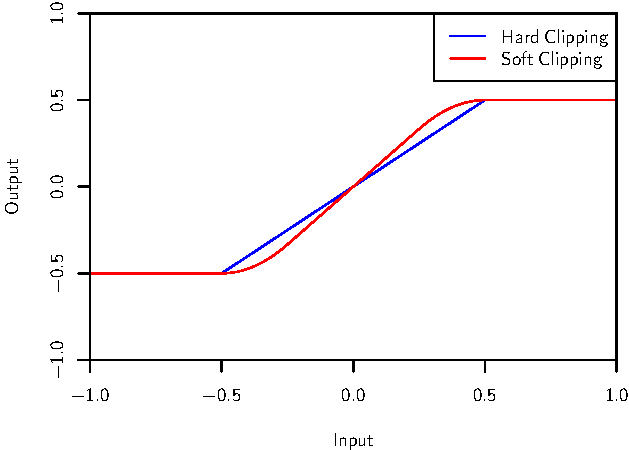
\includegraphics{chapter3/Images/Clipping.pdf}
			\caption{Characteristic curves for \ref{eq:SymmetricHardClipping} and
				 \ref{eq:SymmetricSoftClipping} with a threshold of 0.5.}
			\label{fig:Clipping}
		\end{figure}

	\subsection{Rectification}
	\label{sec:Excitation-Methods-Rectification}
		Rectification is a special case of static nonlinearity. Signals can be either half or full wave rectified,
		as shown in Equations \ref{eq:HalfWaveRectification} and \ref{eq:FullWaveRectification} respectively.

		\begin{equation}
			y[n] = \begin{cases}
				0 & \text{if $x[n] < 0$} \\
				x[n] & \text{otherwise}
			\end{cases}
			\label{eq:HalfWaveRectification}
		\end{equation}

		\begin{equation}
			y[n] = \abs{x[n]}
			\label{eq:FullWaveRectification}
		\end{equation}

	\subsection{Integrator}
	\label{sec:Excitation-Methods-Integrator}
		Equation \ref{eq:Integrator} shows an Integrator adapted from the one described by \citet{larsen2004audio}.

		\begin{equation}
			y[n] = \begin{cases}
				0 & \text{if $x[n] > 0$ and $x[n - 1] \leq 0$} \\
				y[n - 1] + k\abs{x[n]} & \text{otherwise}
			\end{cases}
			\label{eq:Integrator}
		\end{equation}

		Where $k$ is the integration constant, effectively setting the output gain of the system. The output signal
		is reset to 0 ofter every negative to positive zero crossing in order to prevent the sample amplitudes from
		rising indefinitely.

	\subsection{Multiplier}
	\label{sec:Excitation-Methods-Multiplier}
		Multipliers are a subset of static nonlinearities in which input samples are raised to a positive integer
		power as shown in Equation \ref{eq:Multiplier}.

		\begin{equation}
			y[n] = x[n]^{h}, \quad h \in \textbf{N}
			\label{eq:Multiplier}
		\end{equation}

		Exponential distortion extends this method by relaxing the restriction on the exponent ($h$), allowing it
		to take any positive value. The advantages and disadvantages of this will be discussed in this section.

	\subsection{Single Side Band Automodulation}
	\label{sec:Excitation-Methods-SSBA}
		Single sideband automodulation (SSBA) utilises the concept of single sideband modulation
		\citep{corinthios2009signals}. This allows you to apply amplitude modulation to a signal and only produce
		either the sum or difference sideband. This is easily implemented by constructing an analytic signal
		$x_{a}[n]$ from the input signal and raising to a given power to generate harmonics. Equation \ref{eq:SSB}
		shows the $h$\super{th} order single side band automodulation of a signal.

		\begin{equation}
			y[n] = \Re \left( x_{a}[n]^{h} \right), \quad h \in \textbf{N}
			\label{eq:SSB}
		\end{equation}

	\subsection{Instantaneous Amplitude and Phase}
	\label{sec:Excitation-Methods-IAP}
		In this method, the instantaneous amplitude and phase (IAP) of the analytic signal are calculated. These
		values are then used to aid in the construction of harmonics. The instantaneous amplitude of the analytic
		signal is found by taking its absolute value, $\abs{x_{a}[n]}$. The instantaneous phase is found by taking
		the complex argument of the analytic signal, $\arg(x_{a}[n])$. The instantaneous phase can then be scaled
		in order to scale the frequency content of the signal independent of its amplitude. Equation \ref{eq:IAP}
		shows the $h$\super{th} order instantaneous amplitude and phase modulation of a signal.

		\begin{equation}
			y[n] = \abs{x_{a}[n]} \cos \left( h\arg(x_{a}[n]) \right), \quad h \in \textbf{N}
			\label{eq:IAP}
		\end{equation}

	\subsection{Spectral Replication}
	\label{sec:Excitation-Methods-SpectralReplication}
		The principle behind spectral replication is to reproduce the spectral structure of a signal at higher
		frequencies as shown in Figure \ref{fig:SpectralReplication}.

		\begin{figure}[h!]
			\centering
			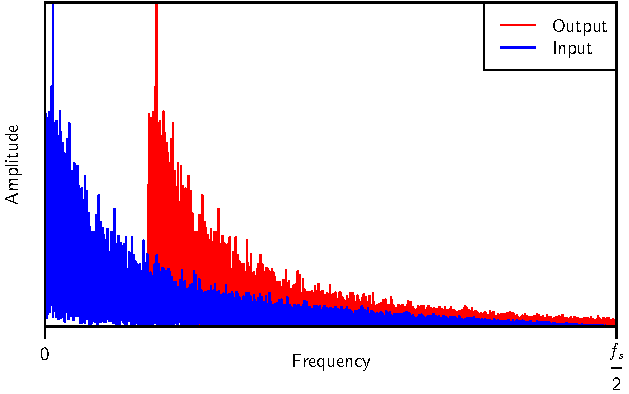
\includegraphics{chapter3/Images/SpectralReplicationSpectrum.pdf}
			\caption{Reproduction of a signal at higher frequencies.}
			\label{fig:SpectralReplication}
		\end{figure}

		This spectral shift is easily implemented through the use of single sideband modulation with a complex
		sinusoid as shown in Equation \ref{eq:SpectralReplication}.

		\begin{equation}
			y[n] = \Re \left( x_{a}[n] e^{2i\pi fn/ f_{s}} \right)
			\label{eq:SpectralReplication}
		\end{equation}

		Where $f$ is the amount by which the signals spectrum should be shifted.

	\subsection{Spectral Folding}
	\label{sec:Excitation-Methods-SpectralFolding}
		Spectral folding uses upsampling in order to replicate parts of the spectrum at higher frequencies. In
		order for the output signal to have the same sampling frequency as the input the signal is 
		downsampled by a factor $k$ before being upsampled by the same factor. 
		
		To avoid aliasing during the downsampling phase the signal should have a low pass filter applied
		with a cutoff frequency of $\frac{f_{s}}{2k}$. Typically upsampling systems apply a low pass filter
		to remove any high frequency content introduced \citep{oppenheim2014discrete}. This is not needed for
		spectral folding as the production of high frequency energy is the desired result.

		After filtering, the downsampling and upsampling can be performed at the same time by retaining
		every $k$\super{th} sample and setting all others to zero. This is shown in Equation
		\ref{eq:SpectralFolding} where $x_{lf}[n]$ is the filtered input signal.		

		\begin{equation}
			y[n] = \begin{cases}
				x_{lf}[n] & \text{if $k \divides n$} \\
				0 & \text{otherwise}
			\end{cases}
			\label{eq:SpectralFolding}
		\end{equation}

	\subsection{Spectral Stretching}
	\label{sec:Excitation-Methods-SpectralStretching}
		The principle of spectral stretching is to scale the spectrum of a signal along the frequency axis. This
		effect is shown in Figure \ref{fig:SpectralStretching}.

		\begin{figure}[h!]
			\centering
			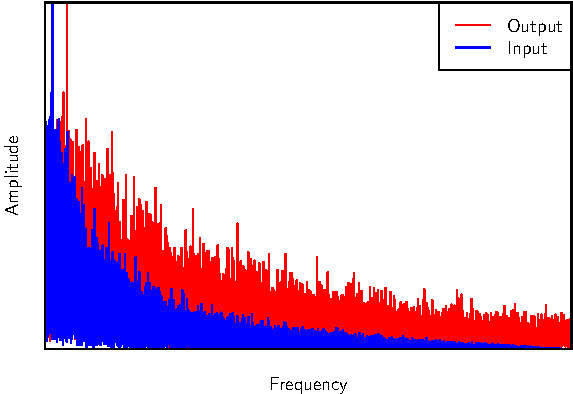
\includegraphics{chapter3/Images/SpectralStretchingSpectrum.pdf}
			\caption{The spectral characteristics of spectral stretching.}
			\label{fig:SpectralStretching}
		\end{figure}

		A typical implementation of this effect utilises a phase vocoder. The phase vocoder is an algorithm which
		allows for time stretching of a signal. It is applied by calculating the short-time Fourier transform of a
		signal with a given frame and hop size. The signal is then resynthesised using a different hop size in
		order to either lengthen or shorten it. This signal can then be resampled back to the length of the
		original signal scaling the frequency content in the process. 
		
		The spectrum is scaled by a factor given in Equation \ref{eq:PhaseVocoderFactor}.

		\begin{equation}
			s = \frac{h_{s}}{h_{a}}
			\label{eq:PhaseVocoderFactor}
		\end{equation}

		Where $h_{a}$ is the hop size used when calculating the STFT and $h_{s}$ is the hop size used to
		resynthesise the signal.

	\subsection{Short-Time Time Reversal}
	\label{sec:Excitation-Methods-STTR}
		Short-Time time reversal (STTR) is an audio effect proposed by \citet{kim2014shorttime}. The output signal
		is constructed from overlapping frames of the input signal which have been reversed in time using Equation
		\ref{eq:STTR}.

		\begin{equation}
			y[n] = \sum_{m = -\infty}^{\infty} w[n - mR]x[2mR - n]
			\label{eq:STTR}
		\end{equation}

		Where $R$ is the step size in samples and $w$ is some window function with constant overlap add (i.e. the
		sum of the window function translated in time by all integer multiples $R$ is one for all values of $n$
		(Equation \ref{eq:ConstantOverlapAdd})).

		\begin{equation}
			\sum_{m = -\infty}^{\infty} w[n - mR] = 1
			\label{eq:ConstantOverlapAdd}
		\end{equation}

		Constant overlap add ensures that no unwanted amplitude modulation is applied to the signal.
